%%%%%%%%%%%%%%%%%%%%%%%%%%%%%%%%%%%%%%%%%%%%%%%%%%%%%%%%%%%
%                                                         %
%       This is documentation for the IPP project.        %
%                                                         %
%%%%%%%%%%%%%%%%%%%%%%%%%%%%%%%%%%%%%%%%%%%%%%%%%%%%%%%%%%%


%------------------------------------------------%
%	    CONFIGURATION + IMPORTED PACKAGES        %
%------------------------------------------------%
\documentclass[10pt,a4paper,titlepage]{article}
\usepackage[english]{babel}
\usepackage[utf8]{inputenc}
\usepackage[margin=100pt]{geometry}


\usepackage{graphicx}   % Import pictures
\usepackage{ragged2e}   % fullfill paragraphs
\usepackage{multicol}
\usepackage{lscape}

\newenvironment{changemargin}[2]{%
\begin{list}{}{%
\setlength{\topsep}{0pt}%
\setlength{\leftmargin}{#1}%
\setlength{\rightmargin}{#2}%
\setlength{\listparindent}{\parindent}%
\setlength{\itemindent}{\parindent}%
\setlength{\parsep}{\parskip}%
}%
\item[]}{\end{list}}

\begin{document}

%-----------------------------------------%
%	              DOCUMENT                  %
%-----------------------------------------%

\setcounter{page}{1}
\pagenumbering{arabic}

\section{IPP project documentation}

\begin{multicols}{2}
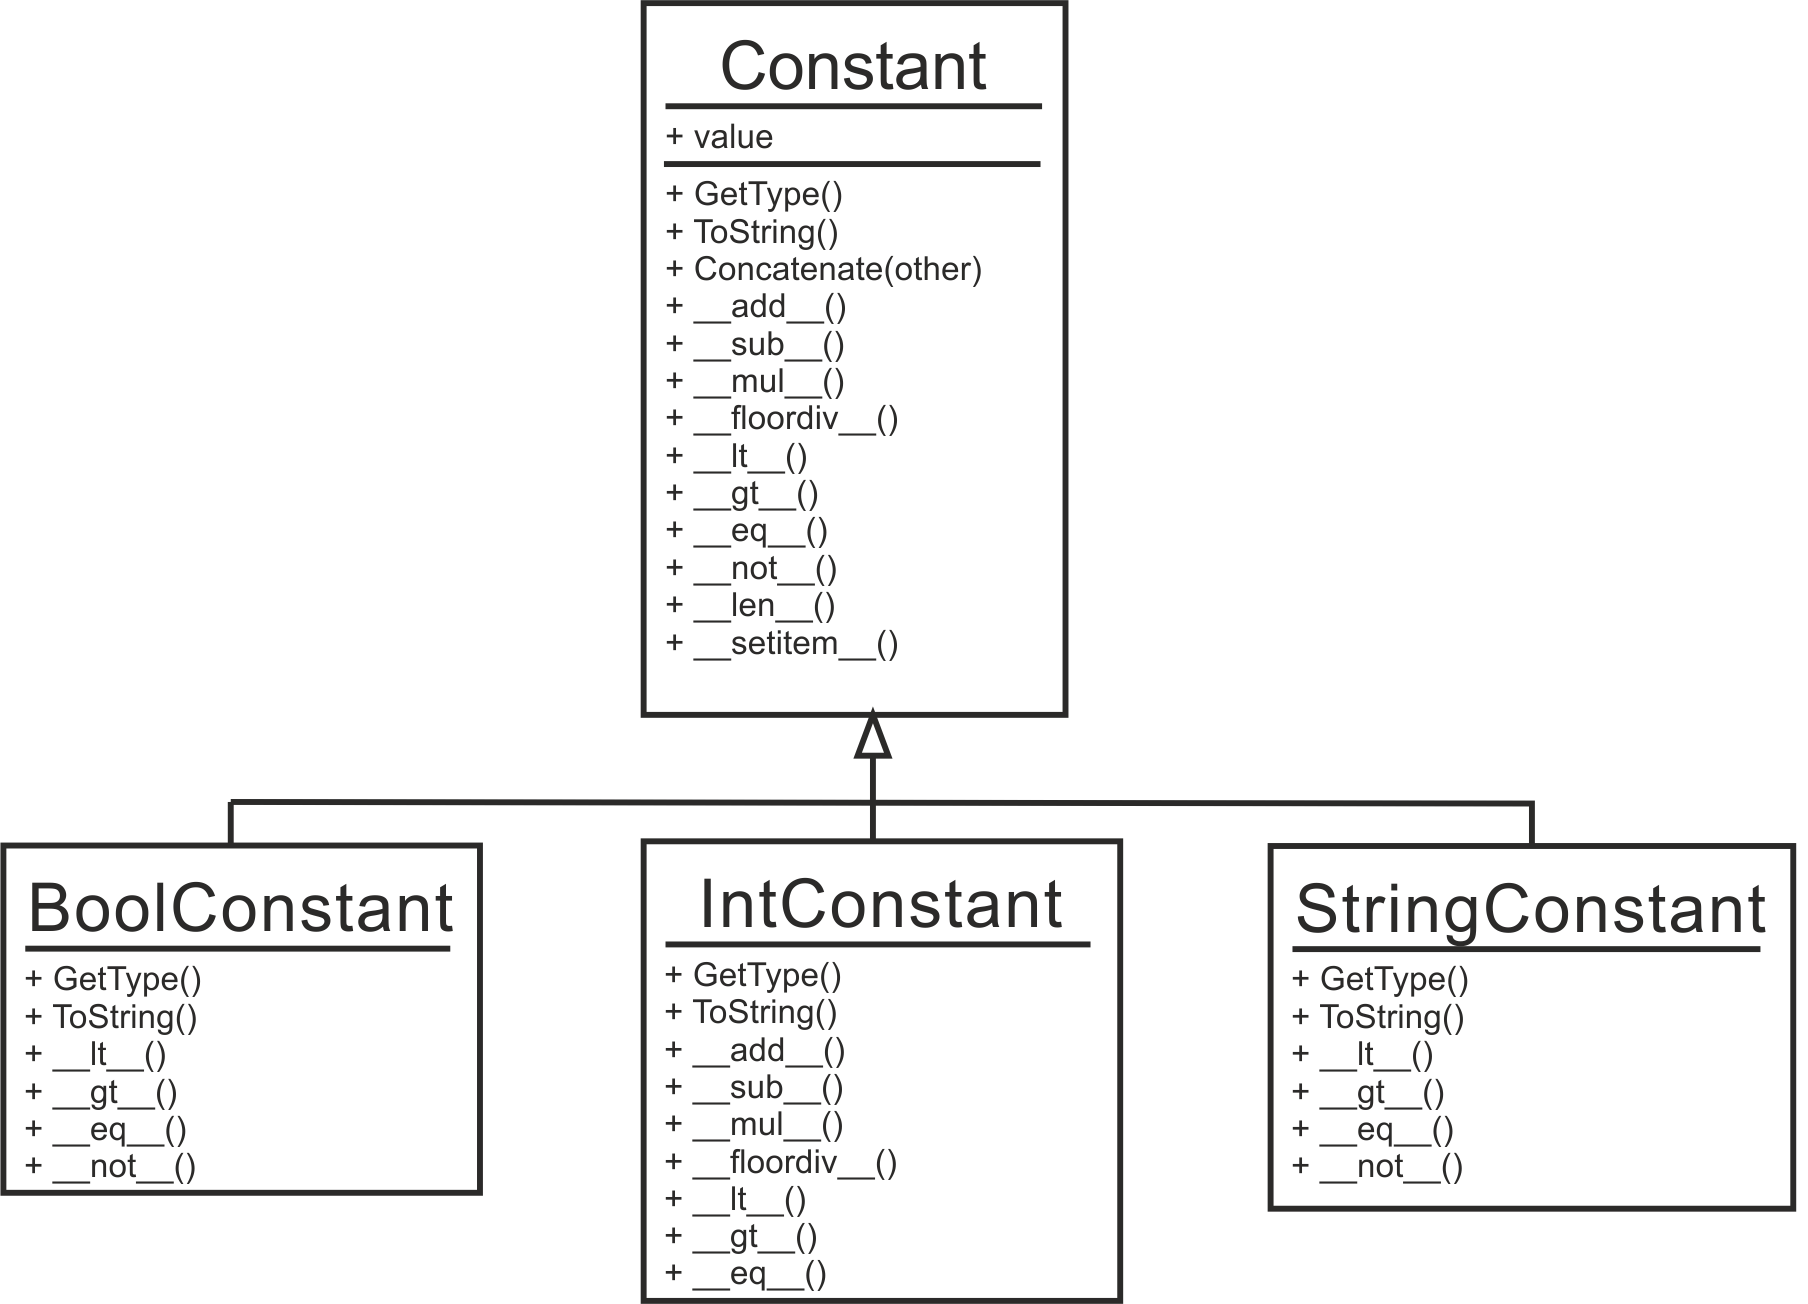
\includegraphics[width=0.45\textwidth]{interpret_constant.png}

\end{multicols}

\paragraph{test.php}
Firstly, it constructs {\it TestSet} and {\it TestConfig} object, that processes
the args and finds the testing files, given to the {\it TestSet} object.

Afterwards, the testing is initiated with {\it Launch()} method of
{\it TestSet} object, receiving {\it Program} object. For each test file,
its method {\it RunTest()} is called. The return value is {\it TestResult}
object, representing the result of testing.

The {\it TestResult} is then analyzed and editted, so the {\it Generator}
object, whom it is given to, could just print the HTML representation with only
a minimum of conditions. It is done at the end of program, printing the
results on standard output in HTML 5 form.

\end{document}
